
\documentclass[twocolumn]{jsarticle}

\usepackage[dvipdfmx]{graphicx}
\usepackage{amsmath}
\usepackage{listings,jlisting}
\usepackage{resume}


\lstset{%
  breaklines=true,
  language=c,
  basicstyle=\ttfamily\small,%
  commentstyle={\itshape},%
  classoffset=1,
  keywordstyle={\bfseries},%
  stringstyle={\ttfamily},
  frame={tbrl},
  framesep=5pt,
  showstringspaces=false,
  numbers=left,%
  stepnumber=1,
  numberstyle=\small,%
  tabsize=4,
  lineskip=-0.5ex,
  linewidth=0.45\textwidth,
  xleftmargin=2zw,
}


\begin{document}
\section{課題1}
\subsection{課題1-1}
プログラミングのツール:BCCにはMAKEユーティリティの他,grepやtouchなどプログラム開発を行う際に役に立つコマンドラインツールが含まれている.それぞれの機能や利用法について学習せよ.

\subsubsection{grep}

テキストファイルから一致する文字列を検索するためのコマンド.
オプションを用いることで行頭や行末を検索するなどの検索法の指定ができる.

\subsubsection{touch}

指定したファイルのタイムスタンプを更新する.オプションを使用することで特定の日時を指定することが可能.指定されたファイルが存在しない場合は新規に作成する.


\subsection{課題1-2}
C 言語:変数の「有効範囲(スコープ)」, 「記憶域期間(記憶寿命)」について学習し,一般的な(ロー
カル)変数とグローバル変数,スタティック変数の違いを整理せよ.

有効範囲とは変数が利用できる範囲のことであり,記憶域機関とは変数がメモリに存在している期間である.
ローカル変数の有効範囲は宣言された関数内である.他の関数でも変数を利用した場合はグローバル変数として宣言すればよい.
ローカル変数は関数が終了するとメモリ上から消去されてしまうが,スタティック変数を用いることでプログラム実行中変数が保存されるようになる.


\subsection{課題1-3}
星型正多角形を描き,回転させるようなプログラムを作成せよ.

星型正多角形を描き回転させるプログラムの主要部をソースコード\ref{src:star}に示す.

\lstinputlisting[caption=星型正多角形描画の主要部, label=src:star]{star.c}

\subsection{課題1-4}
完全グラフを描き,回転させるようなプログラムを作成せよ.

完全グラフを描き回転させるプログラムの主要部をソースコード\ref{src:star}に示す.
各頂点について,まだ線で結ばれていない頂点との線分を描画する処理を行うことで完全グラフを描画した.

\lstinputlisting[caption=完全グラフ描画の主要部, label=src:kanzen]{kanzen.c}

\subsection{課題1-5}
数学関数のグラフを描くプログラムを作成せよ.例えば$\theta$を$0$から$2\pi$まで変化させながら,次の関数をプロットすると
どんな図形が描かれるだろうか.

カージオイドを描画するプログラムの主要部をソースコード\ref{src:gurahu}に示す.
14行から18行までが描画する関数に依存する部分であり,$xy$を媒介変数で表すことで任意の関数を描画できる.

\lstinputlisting[caption=完全グラフ描画の主要部, label=src:gurahu]{gurahu.c}

\section{課題2}
\subsection{課題2-1}
正四面体 $ABCD$について, $\delta BCD$ の重心$G$を原点$O$と一致させ,
$GA$を$x$軸, $GB$を$y$軸とする座標系を考える.正四面体の一辺の長さを$w$とするとき,各頂点の3次元座標を導出せよ.

正四面体の断面図を図\ref{tri}に示す.

\begin{figure}[h]
 \centering
 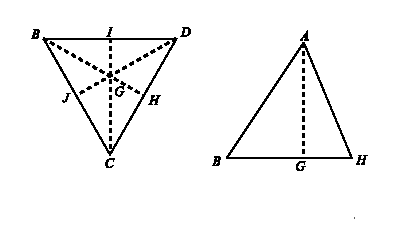
\includegraphics[width=1\hsize]{tri.eps}
\vspace{-13mm}
 \caption{正四面体の断面図}
 \label{tri}
\end{figure}


まず$\triangle{BCD}$を考える.$G$は$BH$を$2:1$に内分する点であり,$BH=\frac{\sqrt{3}}{2}\ w$であるから,

\begin{align*}
GH=\frac{1}{3}\times\frac{\sqrt{3}}{2} w=\frac{\sqrt{3}}{6}\ w\\
GB=\frac{2}{3}\times\frac{\sqrt{3}}{2} w=\frac{\sqrt{3}}{3}\ w
\end{align*}

ここで三平方の定理より,

\begin{align*}
GA=\sqrt{AB^2-GB^2}=\sqrt{w^2-\frac{1}{3}w^2}=\frac{\sqrt{6}}{3}w
\end{align*}

よって各頂点の三次元座標は,

\begin{align*}
点A&:\left(\frac{\sqrt{6}}{3}w, 0, 0\right)&点B&:\left(0, \frac{\sqrt{3}}{3}w, 0\right)\\
点C&:\left(0, -\frac{\sqrt{3}}{6}w, \frac{1}{2}w\right)&点D&:\left(0, -\frac{\sqrt{3}}{6}w, -\frac{1}{2}w\right)
\end{align*}

\subsection{課題2-2}
前問で求めた結果をもとに,原点$O$を中心とする半径$1$の球に内接する正四面体の頂点を導出せよ.

正四面体において,外接球の中心点$G'$と各頂点の間の距離は外接球の半径$r$に等しい.このとき三平方の定理より,

\begin{align*}
G'B^2&=GB^2+G'G^2\\
r^2&=\frac{1}{3}w^2+\bigg(\frac{\sqrt{6}}{3}w-r\bigg)^2\\
r&=\frac{\sqrt{6}}{4}w\\
GG'&=\frac{\sqrt{6}}{12}
\end{align*}

ここで原点$O$と$G'$の位置を合わせるために,$x$軸方向に$-\sqrt{6}/{12}\ w$シフトさせ,$r=1$とすると,

\begin{align*}
点A&:\left(1, 0, 0\right)&点B&:\left(-\frac{1}{3}, \frac{2\sqrt{2}}{3}, 0\right)\\
点C&:\left(-\frac{1}{3}, -\frac{\sqrt{2}}{3}, \frac{\sqrt{6}}{3}\right)&点D&:\left(-\frac{1}{3}, -\frac{\sqrt{2}}{3}, -\frac{\sqrt{6}}{3}\right)
\end{align*}

となる.

\subsection{課題2-3}
アームロボットについて,キー入力で台座の回転と,各関節の傾斜角を制御できるような 対話プログラムを作成してみよう.

アームロボットを回転制御するプログラムの主要部をソースコード\ref{arm}に示す.
keyin関数を用いて台座の回転状態を格納する変数を操作することで,キーボードを用いてアームロボットを制御することができる.

\lstinputlisting[caption=アームロボット制御の主要部, label=arm]{arm.c}

\subsection{課題2-4}
タイマコールバック関数を使って,アームロボットを制御するようなプログラムを作成してみよう.アームロボットが踊っているかのように見せるには,どんな工夫ができるだろうか.

アームロボットを踊らせるプログラムの主要部をソースコード\ref{dance}に示す.
直線的,規則的な動きでは機械感が出てしまい踊っているように見えないと感じたため,乱数を用いて回転させる方法を考えた.
ソースコード\ref{arm}のアームロボット制御プログラムの回転角制御時にこの関数を呼び出すことでランダムに回転するようになる.

\section{課題3}
\subsection{課題3-1}
空間中の任意の3点$P_i=(x_i,y_i,x_i),i=1,2,3$が与えられたとき,$\triangle{P_1P_2P_3}$の単位法線ベクトルをすべて求める式を導出せよ.

ベクトルの外積を用いることで求められる.

外積を求めるため,3点で作られるベクトルのうち2つを考える.
\begin{eqnarray}
\overrightarrow{P_1P_2} = \vec{P_2} - \vec{P_1}\nonumber\\
\overrightarrow{P_2P_3} = \vec{P_3} - \vec{P_2}\nonumber
\end{eqnarray}
この2つのベクトルの外積を計算し,大きさを1とすればよいから,
\begin{equation}
\vec{n}=\pm\frac{\overrightarrow{P_1P_2} \times \overrightarrow{P_2P_3}}{|\overrightarrow{P_1P_2} \times \overrightarrow{P_2P_3}|}\nonumber
\end{equation}

となる.

\subsection{課題3-2}
空間中の任意の3点$P_i=(x_i,y_i,x_i),i=1,2,3$が与えられたとき,$\triangle{P_1P_2P_3}$のどちらが表(CCW)で,どちらが裏(CW)と判定できるか,判定方法を導出せよ.

頂点の順番をあらかじめ定めておき,頂点を時計回りにたどる2つのベクトルの外積ベクトルが向く方向を表(裏)と定めればよい.
カメラから見た時の表裏判別が必要な場合は,カメラからの視線ベクトルを考え,ポリゴンと視線ベクトルの内積を計算する.
外積ベクトルが向く方向を表と定めた場合,カメラからポリゴンの表面が見えているなら,視線ベクトルとポリゴンの外積ベクトルのなす角は90度未満になるため内積は正の値をとる.

\subsection{課題3-3}
phongの照光モデルについて,詳しく調べよ.

phongの照光モデルは,3DCGにおける,モデリングされた面 (surface) 上の点に影をつけるための照明と陰影モデルである.このモデルにおいて反射は,鏡面反射,拡散反射,環境反射の3つで定義される.この3つの反射モデルによって面上の点の陰影を描画する.

まず,光源ごとに鏡面反射成分$i_s$と拡散反射成分$i_d$,アンビエント照明(室内外の環境照明)$i_a$を定義する.次に,光が当たる材質について,鏡面反射係数$k_s$,拡散反射係数$k_d$,環境反射係数$k_a$,光沢度$\alpha$を定義する,そして,光源群に対して,光が当たる点からの位置ベクトル$L$,法線を$N$,光が完全に反射される方向を$R$,光が当たる点から視点に向かう位置ベクトルを$V$とする.これらの定義された情報から,表面上の光の強度$I_p$は次の式で計算できる.

\begin{eqnarray}
I_p &=& k_a i_a + \sum_{Lights}(k_d(L・N)i_d + k_s(R・V)^\alpha i_s) \nonumber
\end{eqnarray}


\subsection{課題3-4}
正四面体,正六面体,正八面体をスムーズシェーディングで表示するために,各頂点の単位法線ベクトルをどのように定めればよいか考え,実装せよ.

正四面体をスムーズシェーディングで表示するためのプログラムの主要部をソースコード\ref{sye}に示す.
頂点が含まれる3つの面の法線ベクトルの平均値をその頂点の法線ベクトルとして実装した.

\lstinputlisting[caption=正四面体スムーズシェーディング表示プログラムの主要部, label=sye]{sye.c}

\subsection{課題3-5}
アームロボットをシェーディング表示するものに変更してみよ.
アームロボットをシェーディング表示するために,アームロボットプログラムに光源を追加するためのソースコードをソースコード\ref{arm2}に示す.

\lstinputlisting[caption=アームロボットシェーディング表示プログラムの追加部, label=arm2]{arm2.c}

\section{感想}
OpenGLの基本事項について理解でき,実装できたので画像処理への理解が深まったと思う.
ただ,複雑な画像処理アプリケーションを実装する際には大変そうだなと感じた.
\section{改善案}
配布資料のPDFファイルに誤植があった.
1.1準備の4.において

glut32.dll:32bitOSではc:\textbackslash Widnows\textbackslash

となっているが,正しくはWindowsだと思われる.

\end{document}




























